\documentclass[12pt]{beamer}
\usetheme[titleformat=allcaps]{metropolis}

% make title separator line invisible
\makeatletter
\setlength{\metropolis@titleseparator@linewidth}{0pt}
\makeatother

% make background color wihite so avatar
% background blend with background color
% \setbeamercolor{background canvas}{bg=white}
\usepackage{appendixnumberbeamer}
\usepackage{url}
\usepackage{minted}
\usepackage{tikz}

% setup default font
% \usefonttheme{serif} % default family is serif
% \usepackage{fontspec}
% \setmainfont{Cochin}


% change bibliography fonts, so references occupy less space on slides
\setbeamerfont{bibliography entry author}{size=\tiny}
\setbeamerfont{bibliography entry title}{size=\tiny}
\setbeamerfont{bibliography entry location}{size=\tiny}
\setbeamerfont{bibliography entry note}{size=\tiny}
\setbeamerfont{bibliography item}{size=\tiny}


\title{Verification of \\ Concurrent and \\ Distributed Systems}
\date{\today}
\author{Nickolai Novik}
\institute{\href{http://github.com/jettify}{http://github.com/jettify}}
\titlegraphic{\hspace*{7cm} 
\includegraphics[height=8.5cm]{figures/avatar3.pdf}}

% =========================================================================== %
\begin{document}
  \maketitle
% --------------------------------------------------------------------------- %
  \begin{frame}{About Me}
    \begin{itemize}
        \item \textbf{[Software Engineer]}  DataRobot
        \item \textbf{[Github]}
            \href{http://github.com/jettify}{http://github.com/jettify}
        \item \textbf{[Twitter]}
            \href{https://twitter.com/isinf}{https://twitter.com/isinf}
        \item \textbf{[aio-libs]}
            \href{https://github.com/aio-libs}{https://github.com/aio-libs}
        \item \textbf{[Projects]}
            \textit{aiomonitor, aiohttp-debugtoolbar,
          aiobotocore, aiomysql, aioodbc, aiohttp-admin, aiorwlock,
          aiozipkin, etc}
    \end{itemize}
  \end{frame}
% --------------------------------------------------------------------------- %
%  \begin{frame}[squeeze]{Agenda}
%      \setbeamertemplate{section in toc}[sections numbered]
%      \tableofcontents
%  \end{frame}
% --------------------------------------------------------------------------- %
  \begin{frame}{Poll}
      \begin{large}
          \textbf{How many of you heard of formal methods?}
      \end{large}
      \begin{itemize}
          \item I used one on of: Coq, Isable, TLA+, Alloy, Spin.
          \item I heard about it, but never used.
          \item I think formal methods are kinda cool.
      \end{itemize}
  \end{frame}
% --------------------------------------------------------------------------- %
  \section{Problem Statement. Motivational Example}
% --------------------------------------------------------------------------- %
  \begin{frame}{Concurrent and Distributed systems \\ are hard}
      \textbf{Most of industry uses following techniques for quality assurance:}
      \begin{itemize}
          \item Design review
          \item Code review
          \item Unit/Integration/Functional testing
          \item Static code analysis
          \item Code coverage
          \item Stress testing
          \item Fault-injection testing \cite{principlesofchaos}
      \end{itemize}
  \end{frame}
% --------------------------------------------------------------------------- %
  \begin{frame}{Distributed algorithms extremely hard}
      \begin{center}
          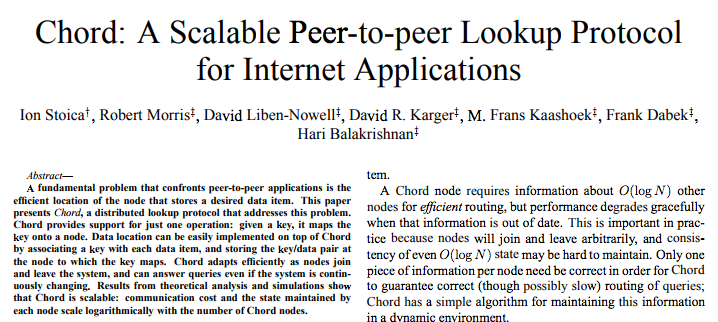
\includegraphics[scale=0.3]{figures/chord_paper.png}
      \end{center}
      \begin{alertblock}{Chord}
          is popular algorithm for P2P systems, paper published in
          2001 by strong team of MIT researchers, 10 years later bug found
          in specification~\cite{stoica2001chord, Zave15}. Paper won best
          paper award.
      \end{alertblock}
  \end{frame}
% --------------------------------------------------------------------------- %
%  \begin{frame}{Sometimes cost of error is very high}
%      \begin{center}
%          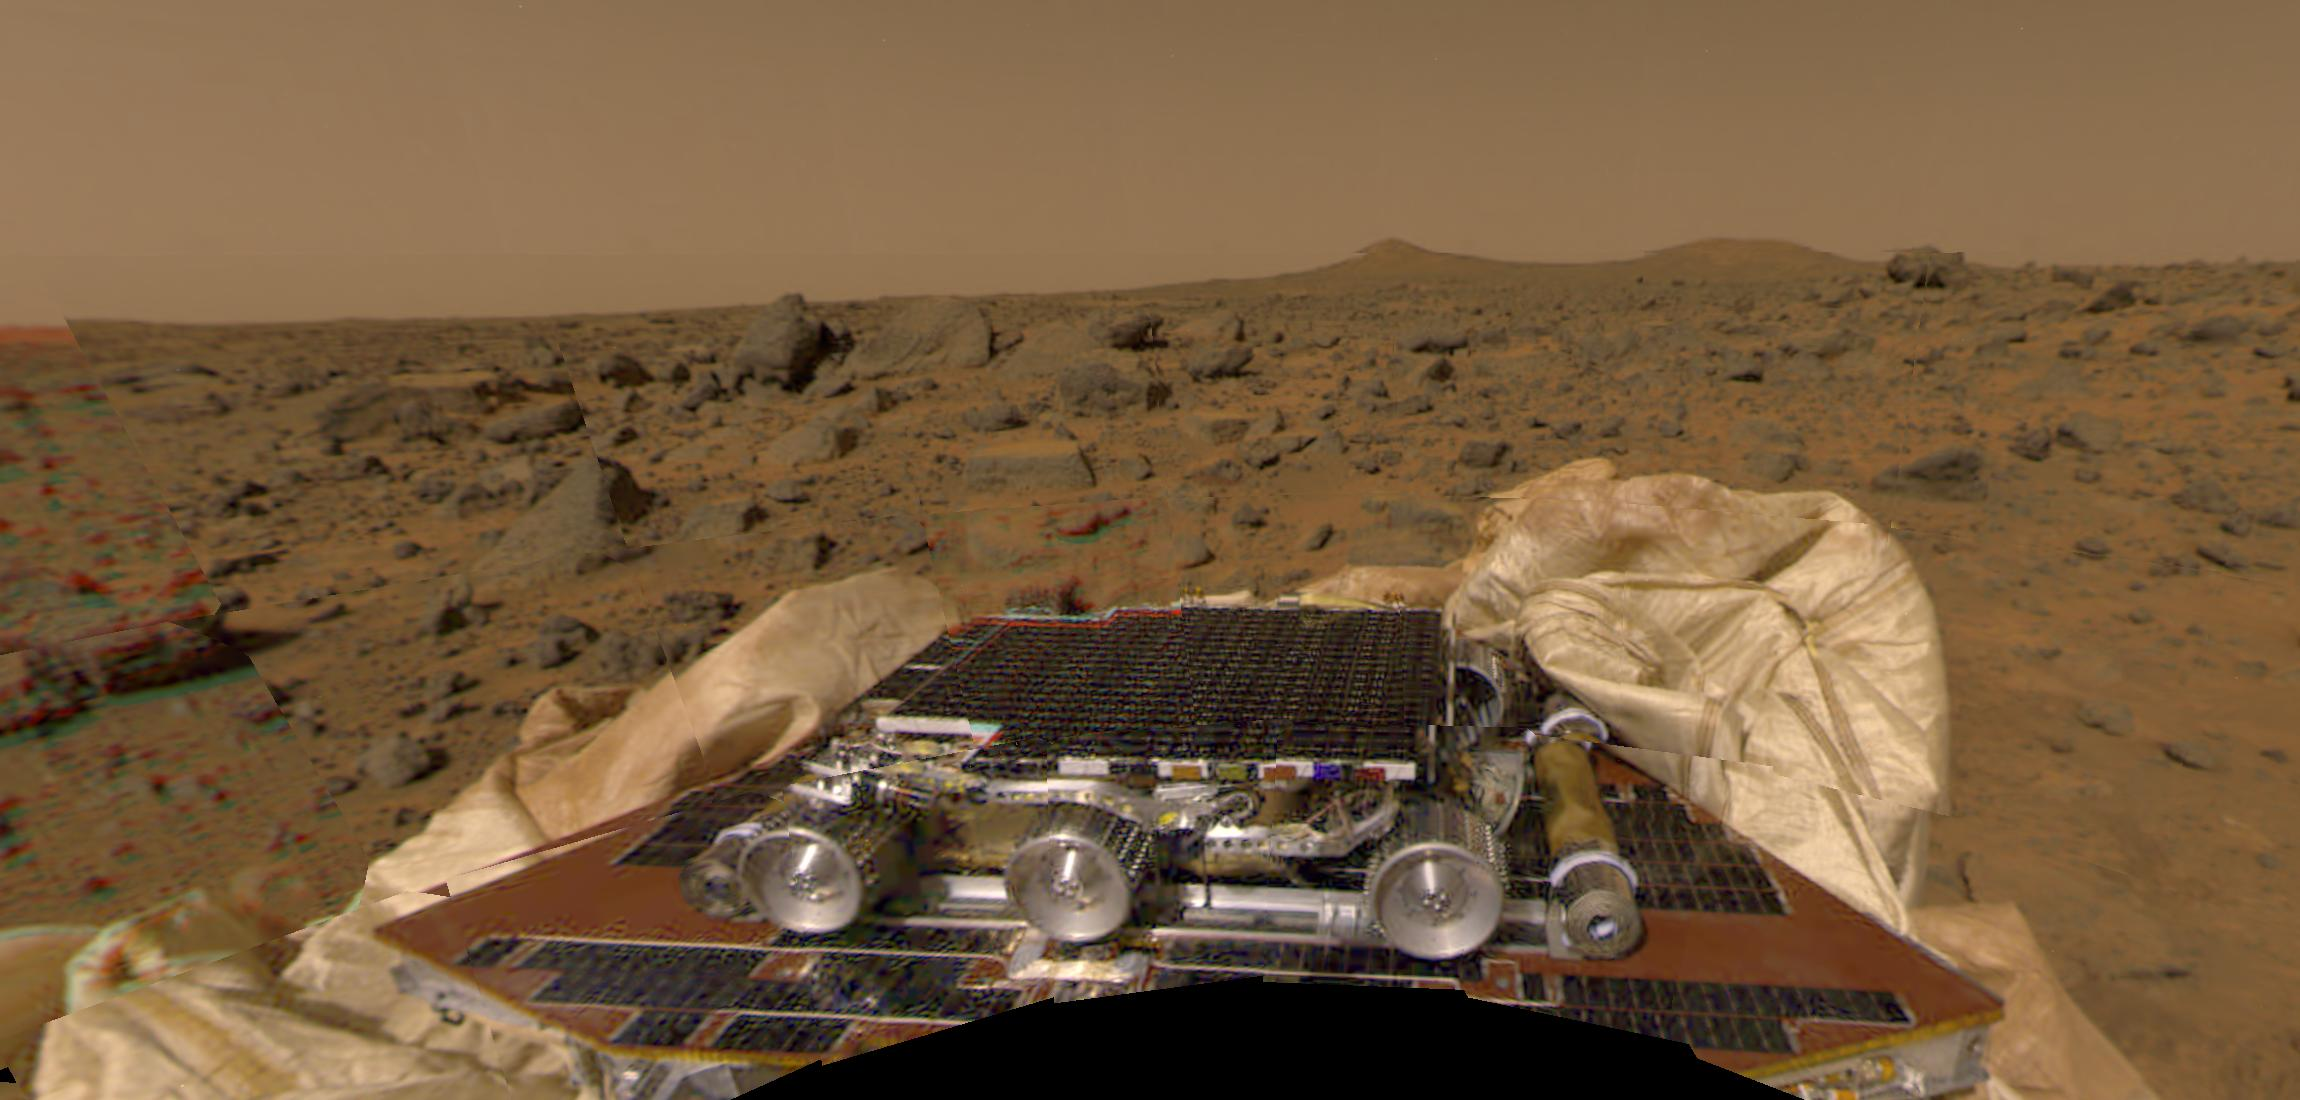
\includegraphics[scale=0.12]{figures/pathfinder.jpg}
%      \end{center}
%      \begin{alertblock}{Mars Pathfinder}
%          rover, the mission was jeopardised by a concurrent
%          software bug in the lander.~\cite{Pathfinder2013}
%      \end{alertblock}
%  \end{frame}
% --------------------------------------------------------------------------- %
  \begin{frame}{Sometimes cost of error is very high 2}
      \begin{center}
          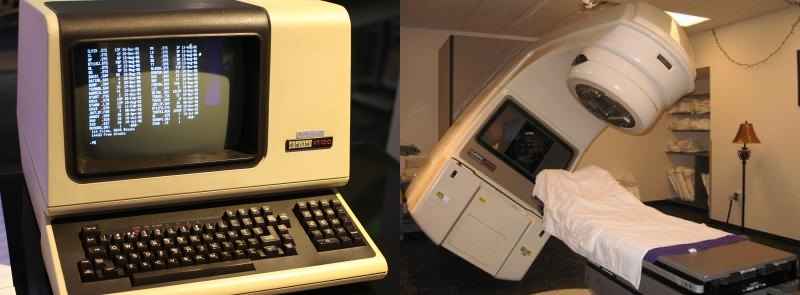
\includegraphics[scale=0.5]{figures/therac.jpg}
      \end{center}
      \begin{alertblock}{Therac-25}
          radiation therapy machine, because of concurrent
          programming errors, it sometimes gave its patients radiation doses
          that were hundreds of times greater than normal~\cite{wiki:therac}
      \end{alertblock}
  \end{frame}
% --------------------------------------------------------------------------- %
  \section{Formal Methods}
% --------------------------------------------------------------------------- %
  \begin{frame}{Formal Methods}
    \textbf{Formal Methods} - are a particular kind of mathematically based
      techniques for the specification, development and verification of
      software systems \cite{mit2002}.
      \begin{center}
          \begin{tikzpicture}[sibling distance=10em, every node/.style = {
                  shape=rectangle, rounded corners, draw, align=center,
                  top color=white, bottom color=blue!5}]]
              \node {Formal Methods}
                child {node {Formal Spec}}
                child {node {Formal Proof}}
                child {node {Model checking} };
          \end{tikzpicture}
      \end{center}
  \end{frame}
% --------------------------------------------------------------------------- %
  \begin{frame}{Model checking}
      \textbf{Model checking} is a technique for automatically verifying
      correctness properties of finite-state systems.
      \begin{center}
          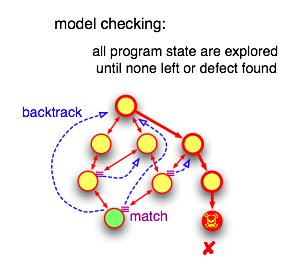
\includegraphics[scale=0.5]{figures/states-mc.png}
          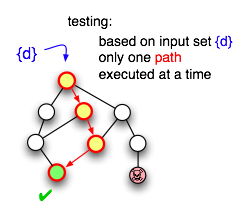
\includegraphics[scale=0.6]{figures/states-testing.png}
      \end{center}
  \end{frame}
% --------------------------------------------------------------------------- %
  \begin{frame}{TLA+ -- Temporal Logic of Actions}
      \begin{center}
          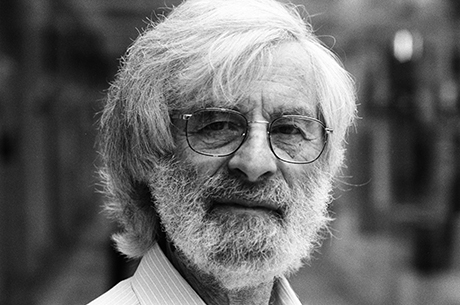
\includegraphics[scale=0.3]{figures/lamport.jpg}
      \end{center}
      \textbf{TLA+} language developed by \textbf{Leslie Lamport}. It is
      used to design, model, document, and verify concurrent systems, has
      been described as exhaustively-testable pseudocode and blueprints
      for software systems.
  \end{frame}
% --------------------------------------------------------------------------- %
  \begin{frame}{TLA+ Description}
      \textbf{TLA+} is \textbf{specifications} language, it is precise written
      description of what a system suppose to do. \textbf{TLA Toolbox}
      distribution of TLA related tools. \textbf{TLC} - model checker
      tool to validate invariants stated in spec. \textbf{TLAPS} - mechanical
      proof checker.

      \begin{description}[align=right]
        \item [Released] April 23, 1999; 18 years ago
        \item [Syntax] math notation, similar to \LaTeX
        \item [Implem.] Java
        \item [License] MIT
        \item [IDE] TLA Toolbox (Eclipse based) \cite{azurewebsites}
      \end{description}
  \end{frame}
% --------------------------------------------------------------------------- %
  \begin{frame}{TLA+ industry usage: AWS}
    \begin{center}
       
\includegraphics[scale=0.08]{figures/aws}
    \end{center}
      \textbf{TLA+} helped to find design bugs in \textbf{S3, Dynamo, EBS, EC2},
      etc, some requiring traces of 35 steps.~\cite{aws2014}
  \end{frame}
% --------------------------------------------------------------------------- %
  \begin{frame}{TLA+ industry usage: Microsoft}
      MS used TLA+ to define consistency protocol for CosmosDB and memory
      allocator for XBox~\cite{ms2017}
    \begin{center}
        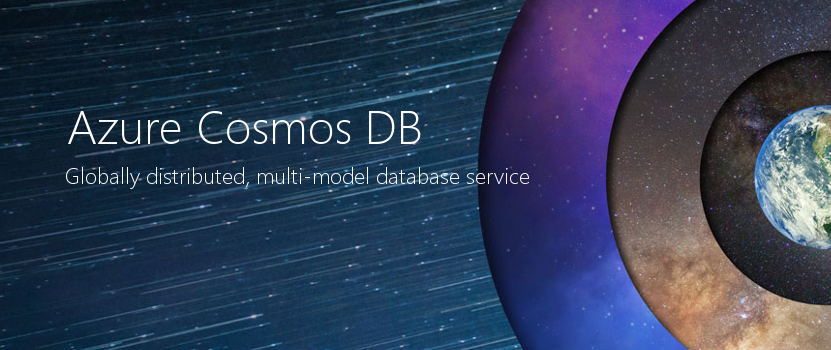
\includegraphics[scale=0.2]{figures/cosmos}
    \end{center}
    \begin{center}
        
\includegraphics[scale=0.2]{figures/xbox}
    \end{center}
  \end{frame}
% --------------------------------------------------------------------------- %
  \begin{frame}{TLA+ industry usage: Open-source}
      Open source projects use TLA+ to verify algorithms:
    \begin{itemize}
        \item \textbf{Linux Kernel} -- verify fairness of qspinlock ~\cite{lkml2018}
        \item \textbf{Elastic} -- data replication protocol~\cite{elastic2017}
        \item \textbf{Mongodb} -- data replication protocol~\cite{mongo2016}
        \item \textbf{Hadoop/YARN} -- registry of long lived processes~\cite{hadoop2017}
    \end{itemize}
    \begin{center}
        
\includegraphics[scale=0.07]{figures/tux}
        
\includegraphics[scale=0.1]{figures/mongo}
    \end{center}
    \begin{center}
        
\includegraphics[scale=0.12]{figures/elastic}
        
\includegraphics[scale=0.14]{figures/hadoop}
    \end{center}
  \end{frame}
% --------------------------------------------------------------------------- %
%  \begin{frame}{RAFT and TLA+}
%    \begin{center}
%          \inputminted[firstline=452,lastline=461,linenos,
%            fontsize=\scriptsize]{tla}{figures/raft.tla}
%    \end{center}
%      RAFT - core algorithm of \textbf{consul}, \textbf{etcd} also verified
%      with TLA+.
%  \end{frame}
% --------------------------------------------------------------------------- %
  \section{TLA+ Basics}
% --------------------------------------------------------------------------- %
  \begin{frame}{TLA+ hello worlds}
    \begin{center}
      \inputminted[linenos,fontsize=\scriptsize]{tla}{figures/hourclock.tla}
      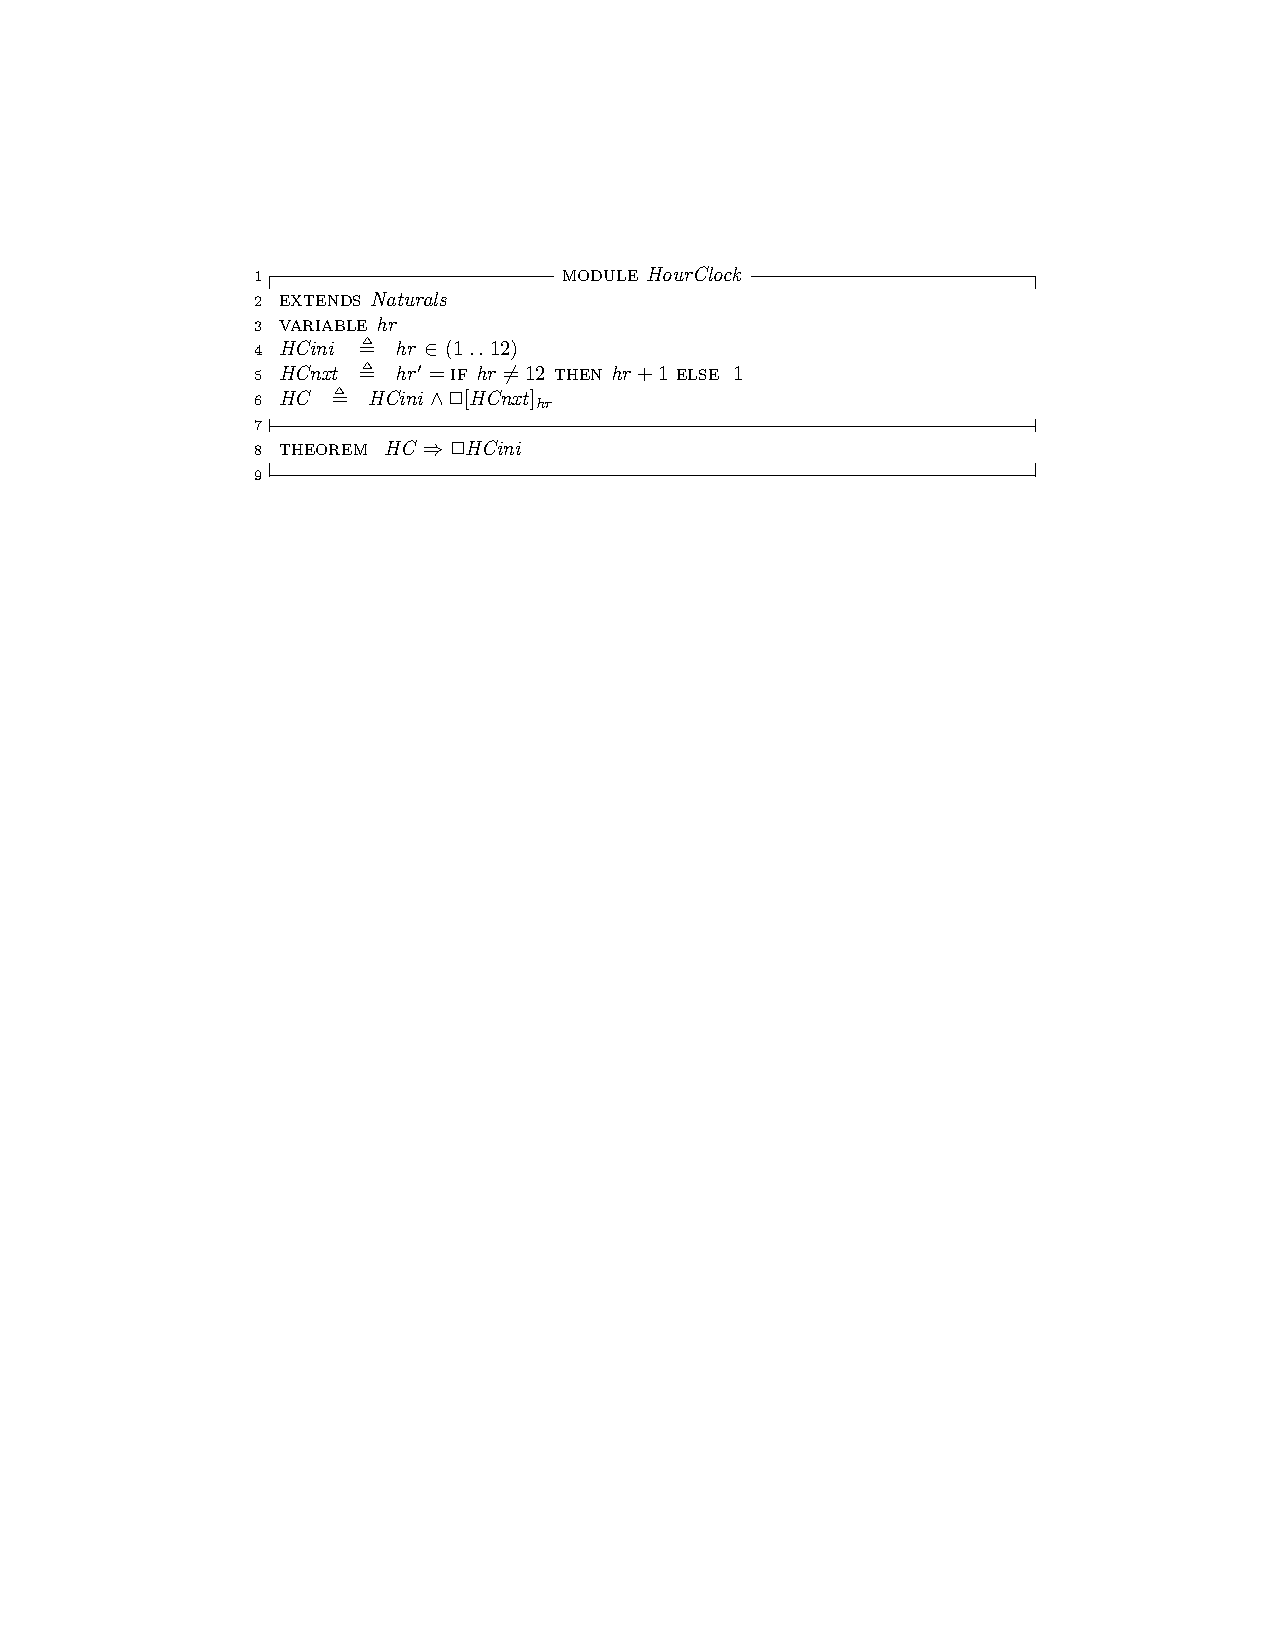
\includegraphics[scale=0.8]{figures/hourclock.pdf}
    \end{center}
  \end{frame}
% --------------------------------------------------------------------------- %
  \begin{frame}{TLA+ syntax. Logic}
      Basic logical operators:
        \begin{table}
        \centering
            \begin{tabular}{@{} lllp{7cm} @{}}
                Symb.         & ASCII                       & Python & Description   \\ \hline
                $\lor$        & \texttt{\textbackslash /}   & \mintinline{python}{or} &logical OR \\
                $\land$       & \texttt{/\textbackslash}   & \mintinline{python}{and} &logical AND \\
                $\lnot$       & \texttt{\~}                  & \mintinline{python}{not} &logical NOT \\
                $=$           & \texttt{=}                  & \mintinline{python}{==} & boolean operator, checks equality, it is not an assignment operator. \\
                $\triangleq$  & \texttt{==}                 & \mintinline{python}{=} & means defined to equal.

            \end{tabular}
        \end{table}
  \end{frame}
% --------------------------------------------------------------------------- %
  \begin{frame}{Exercise}
    \begin{center}
        $ \only<1>{FALSE \land}\only<2>{\boxed{FALSE \land}} (TRUE \land (FALSE \lor TRUE) \lor (TRUE \lor FALSE)) =  \boxed{\only<1>{??}\only<2>{FALSE}}$
    \end{center}
  \end{frame}
% --------------------------------------------------------------------------- %
  \begin{frame}{TLA+ syntax. More Logic}
      More logic operators:
        \begin{table}
        \centering
            \begin{tabular}{@{} lllp{7cm} @{}}
                Symb.     & ASCII                     & Python                     & Description   \\ \hline
                $\exists$ & \texttt{\textbackslash E} & \mintinline{python}{any()} & means "there exists"\\
                $\forall$ & \texttt{\textbackslash A} & \mintinline{python}{all()} & means "for all"\\
                $:$       & $:$                       &                            & reads as "such that"
            \end{tabular}
        \end{table}

      $\exists x \in {1,2,3,4,5} : x > 3$ - exists $x$ in
      set of integers ${1,2,3,4,5}$ such that $x > 3$ expression evaluates
      to TRUE.
  \end{frame}
% --------------------------------------------------------------------------- %
  \begin{frame}{TLA+ syntax. More Logic}
      More logic operators:
        \begin{table}
        \centering
            % \begin{tabular}{|l|p{9cm}|}
            \begin{tabular}{@{} llp{9cm} @{}}
                Operator    & ASCII       & Description   \\ \hline
                $\square$   & \texttt{[]} & formula is TRUE on each step  \\
                $\implies$  & \texttt{=>} & implication \mintinline{python}{x_imp_y = y if x else True}\\
                \boxed{$'$} & \texttt{'}  & reads as prime, state of variable on \\
                            &             & next step \mintinline{latex}{x' = x + 1}\\
            \end{tabular}
        \end{table}
            % \texttt{Init /\textbackslash [][Next]\_hr} formula true on each steup for temporal variable \texttt{hr}
  \end{frame}
% --------------------------------------------------------------------------- %
  \begin{frame}{TLA+ syntax. Sets}
      Basic set operations:
        \begin{table}
        \centering
            \begin{tabular}{@{} lllp{7cm} @{}}
                Symb.           & ASCII                              & Python                                & Description   \\ \hline
                $S \cup T$      & \texttt{\textbackslash union}      &\mintinline{python}{s.union(t)}        & Union\\
                $S \cap T$      & \texttt{\textbackslash intersect}  &\mintinline{python}{s.intersection(t)} & Intersection \\
                $S \subseteq T$ & \texttt{\textbackslash supseteq}   &\mintinline{python}{s in t}            & Membership  \\
                $S \setminus T$ & \texttt{\textbackslash}            &\mintinline{python}{s.difference(t)}   & Difference \\
            \end{tabular}
        \end{table}
  \end{frame}
% --------------------------------------------------------------------------- %
  \begin{frame}{TLA+ Spec Template}
      \begin{center}
          \inputminted[linenos, fontsize=\scriptsize]{tla}{figures/template.tla}
      \end{center}
  \end{frame}
% --------------------------------------------------------------------------- %
  \section{Multithreading Queue Spec}
% --------------------------------------------------------------------------- %
  \begin{frame}{Multithreading Queue}
      Classic \textit{bounded buffer}, attempts to put an element into a
      full queue or take from empty will block.
      \begin{center}
          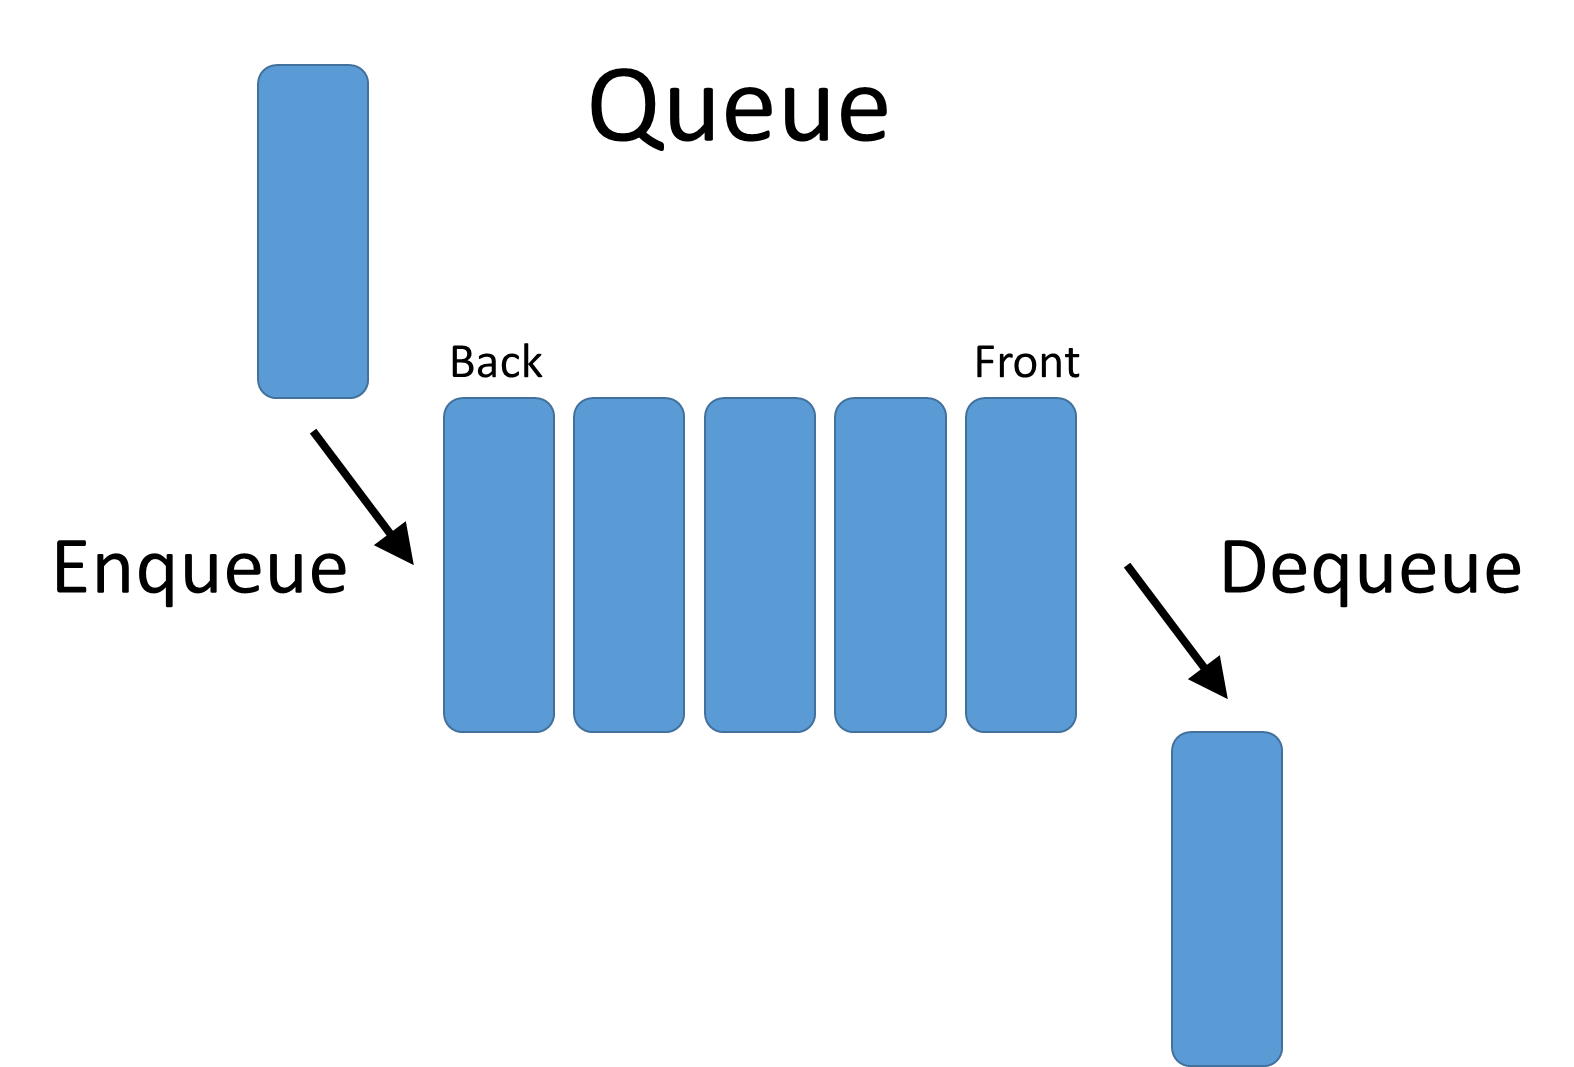
\includegraphics[scale=0.30]{figures/queue}
      \end{center}
  \end{frame}
% --------------------------------------------------------------------------- %
  \begin{frame}{Queue implementation, part 1}
      \begin{center}
          \inputminted[firstline=1,lastline=20,linenos,
            fontsize=\scriptsize]{python}{figures/queue.py}
      \end{center}
  \end{frame}
% --------------------------------------------------------------------------- %
  \begin{frame}{Queue implementation, part 2}
      \begin{center}
          \inputminted[firstline=22,lastline=40,linenos,
            fontsize=\scriptsize]{python}{figures/queue.py}
      \end{center}
  \end{frame}
% --------------------------------------------------------------------------- %

  {\usebackgroundtemplate{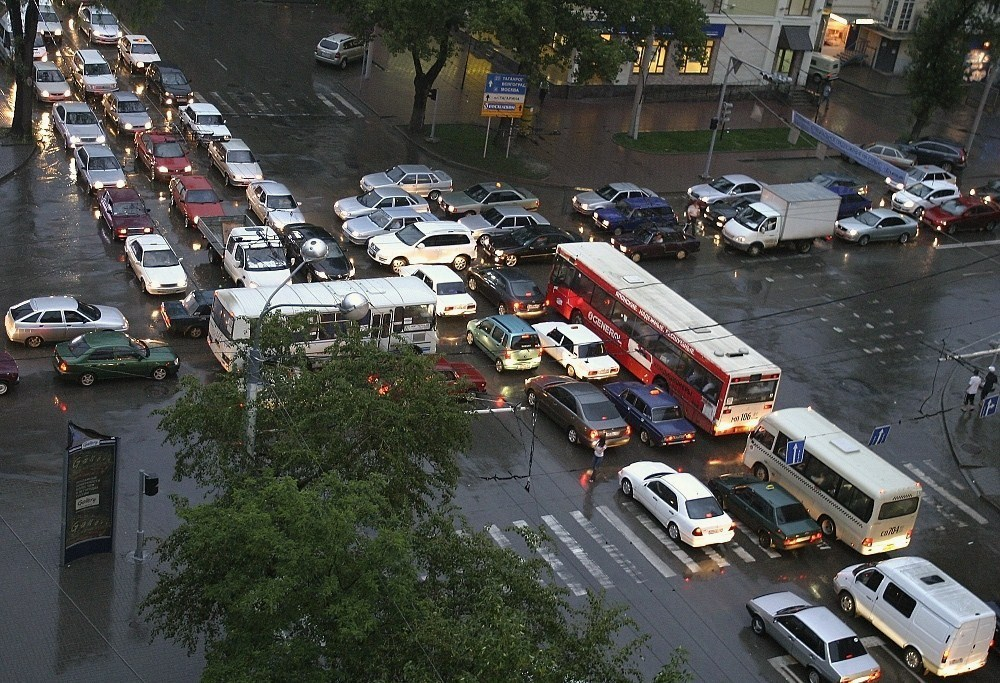
\includegraphics[width=\paperwidth]{figures/deadlock}}
  \begin{frame}{Can you guess type of bug?}
      \begin{center}
      \end{center}
  \end{frame}}
% --------------------------------------------------------------------------- %
  \begin{frame}{Queue TLA spec: part 1}
      \begin{center}
          \inputminted[firstline=1,lastline=16,linenos,
            fontsize=\scriptsize]{tla}{figures/buffer.tla}
      \end{center}
  \end{frame}
% --------------------------------------------------------------------------- %
  \begin{frame}{Queue TLA spec: part 2}
      \begin{center}
          \inputminted[firstline=16,lastline=31,linenos,
            fontsize=\scriptsize]{tla}{figures/buffer.tla}
      \end{center}
  \end{frame}
% --------------------------------------------------------------------------- %
  \begin{frame}{Queue TLA spec: part 3}
      \begin{center}
          \inputminted[firstline=32,lastline=42,linenos,
            fontsize=\scriptsize]{tla}{figures/buffer.tla}
      \end{center}
  \end{frame}
% --------------------------------------------------------------------------- %
  \begin{frame}{Queue TLA spec: part 4}
      \begin{center}
          \inputminted[firstline=43,lastline=50,linenos,
            fontsize=\scriptsize]{tla}{figures/buffer.tla}
      \end{center}
      Invariant definition
  \end{frame}
% --------------------------------------------------------------------------- %
  \begin{frame}{Queue trace}
      TLC shows all steps that leads to \textit{invariant violation}.
      \begin{center}
          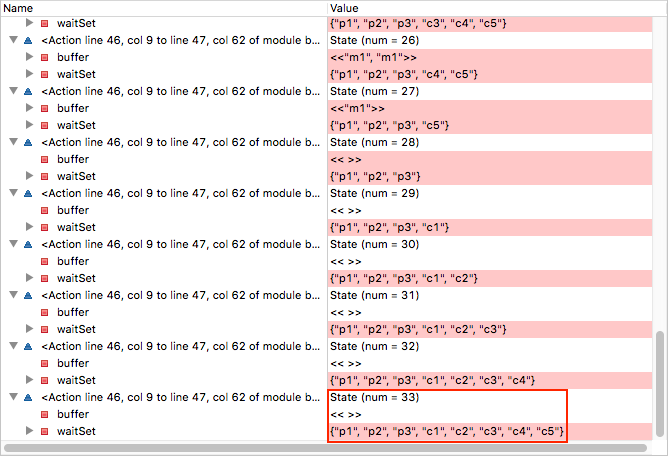
\includegraphics[scale=0.42]{figures/buffer_trace}
      \end{center}
  \end{frame}
% --------------------------------------------------------------------------- %
  \begin{frame}{The Bug}
    \begin{itemize}
      \item Condition variable shared between producers and consumer
      \item On producer signal other producer make wake up instead of consumer
      \item Bug is very hard to reproduce since 30 specific steps need to happen
      \item \textit{NotifyAll} strategy fixes issue with deadlock.
      \item If number of threads > 2 * buffer capacity algorithm is not deadlock free.
    \end{itemize}
  \end{frame}
% --------------------------------------------------------------------------- %
  \begin{frame}{notify\_all() vs notify()}
    \begin{columns}[T] % align columns
      \begin{column}{.48\textwidth}
        \begin{center}
            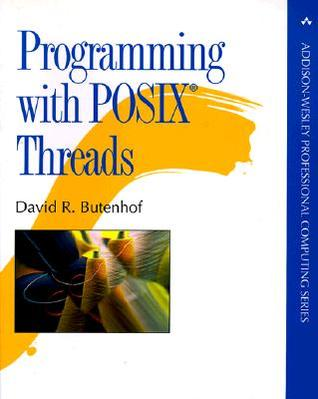
\includegraphics[scale=3.0]{figures/posix_threads}
        \end{center}
      \end{column}%
      \begin{column}{.48\textwidth}
          If ..., you \textbf{share a condition variable} between multiple
          predicates, you \textbf{must always broadcast}, never signal; \\
          \textit{Book: Programming with POSIX Threads by David R. Butenhof}
      \end{column}%
    \end{columns}
  \end{frame}
% --------------------------------------------------------------------------- %
  \section{Aiorwlock Spec}
% --------------------------------------------------------------------------- %
  \begin{frame}[fragile]{aiorwlock~-- read write lock for \\ asyncio}
      An RW lock allows concurrent access for read-only operations,
      while write operations require exclusive access, simple example:
      \inputminted[linenos,fontsize=\scriptsize]{python}{figures/lock.py}
  \end{frame}
% --------------------------------------------------------------------------- %
%  \begin{frame}{aiorwlock~-- bug}
%      \begin{center}
%        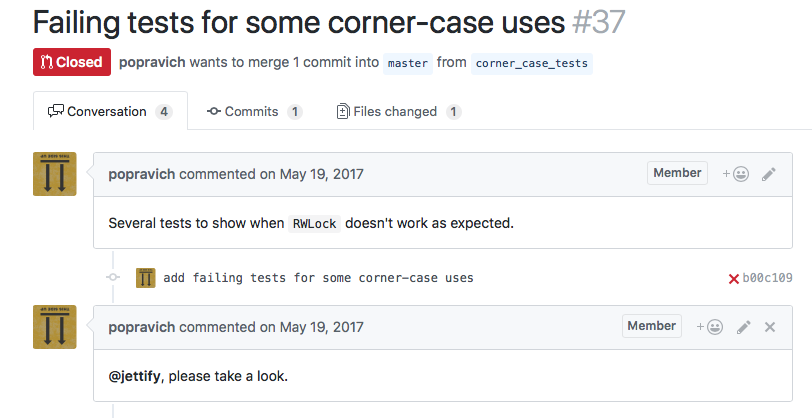
\includegraphics[scale=0.40]{figures/aiorwlock_bug}
%      \end{center}
%  \end{frame}
% --------------------------------------------------------------------------- %
%  \begin{frame}{aiorwlock possible states}
%      Read Write lock state machine:
%      \begin{center}
%          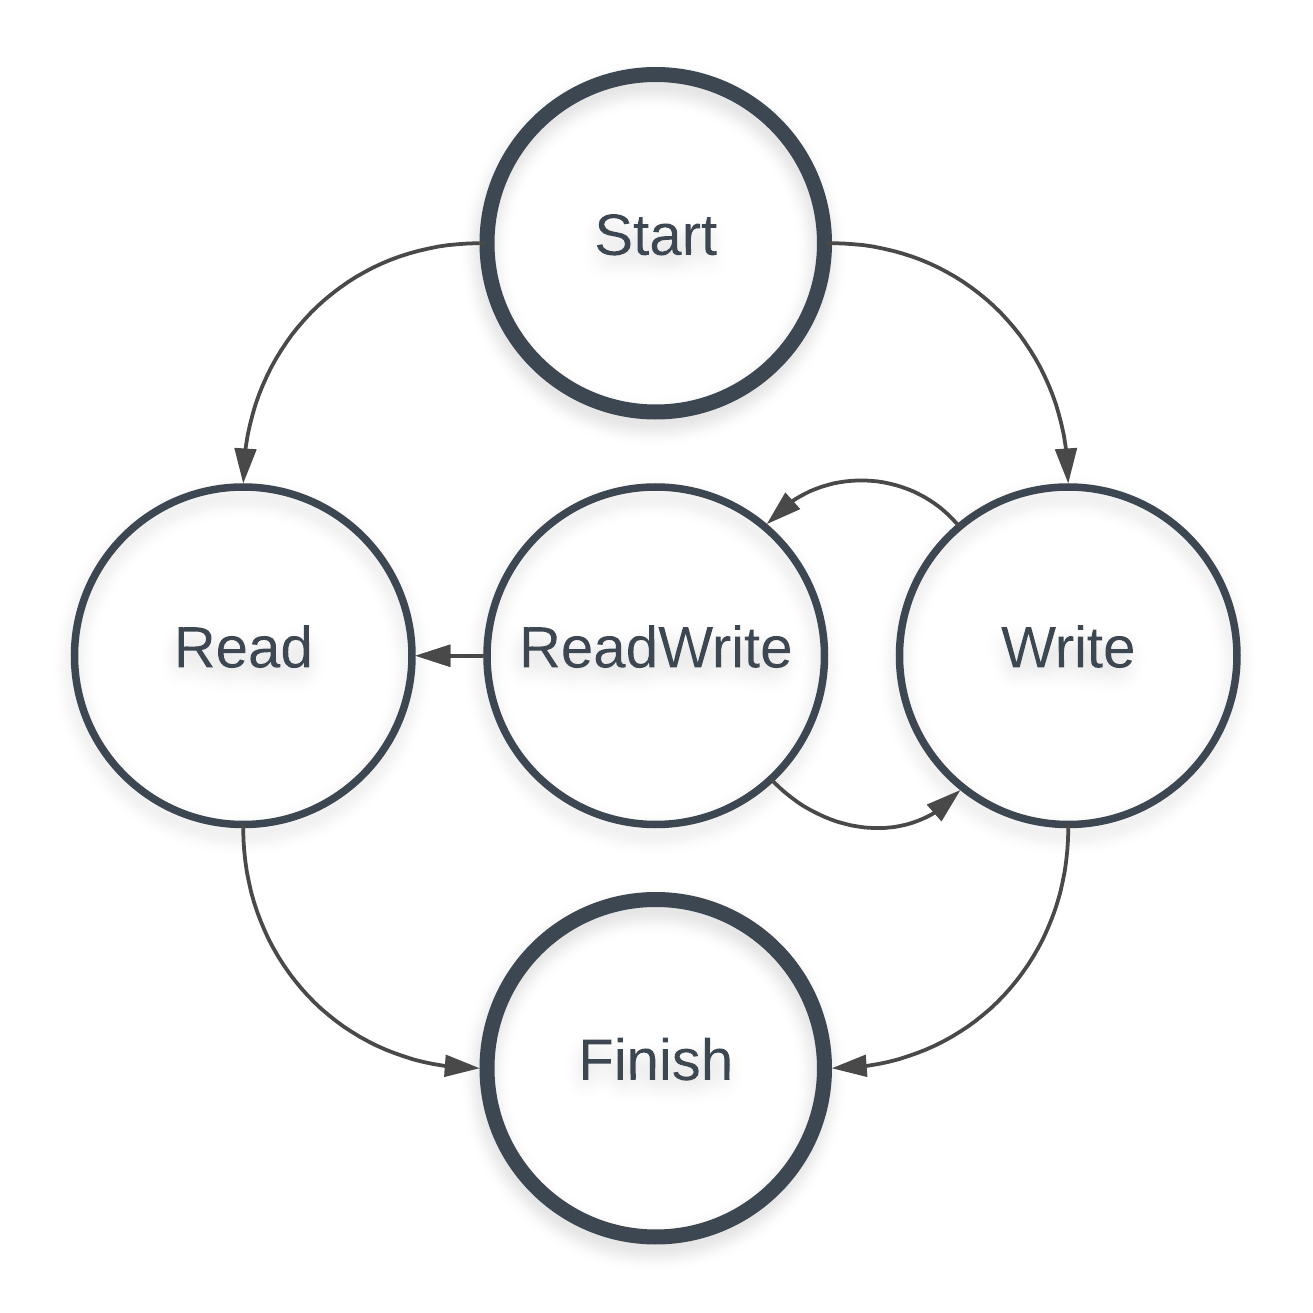
\includegraphics[scale=0.15]{figures/task_states2}
%      \end{center}
%  \end{frame}
% --------------------------------------------------------------------------- %
  \begin{frame}{aiorwlock trace}
      \begin{center}
          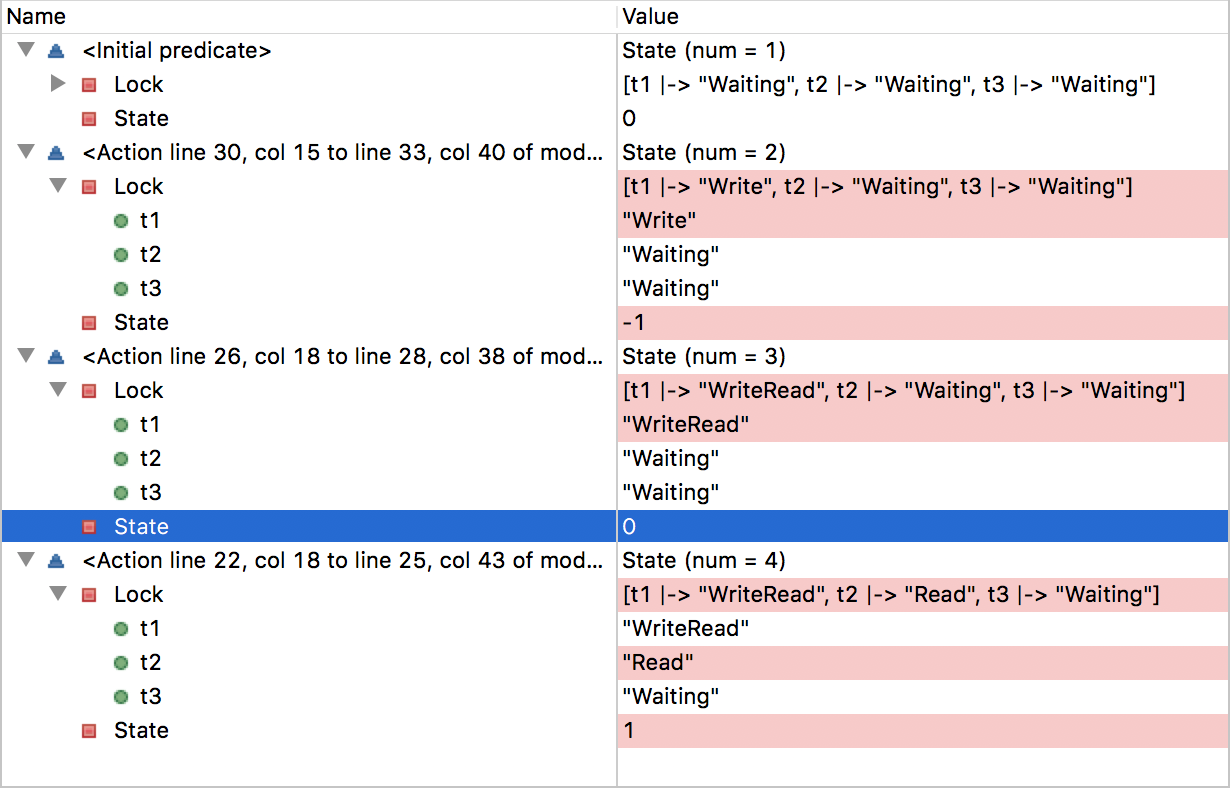
\includegraphics[scale=0.50]{figures/tla_trace}
      \end{center}
  \end{frame}
% --------------------------------------------------------------------------- %
  \begin{frame}{aiorwlock possible states for 2 tasks}
      \begin{center}
          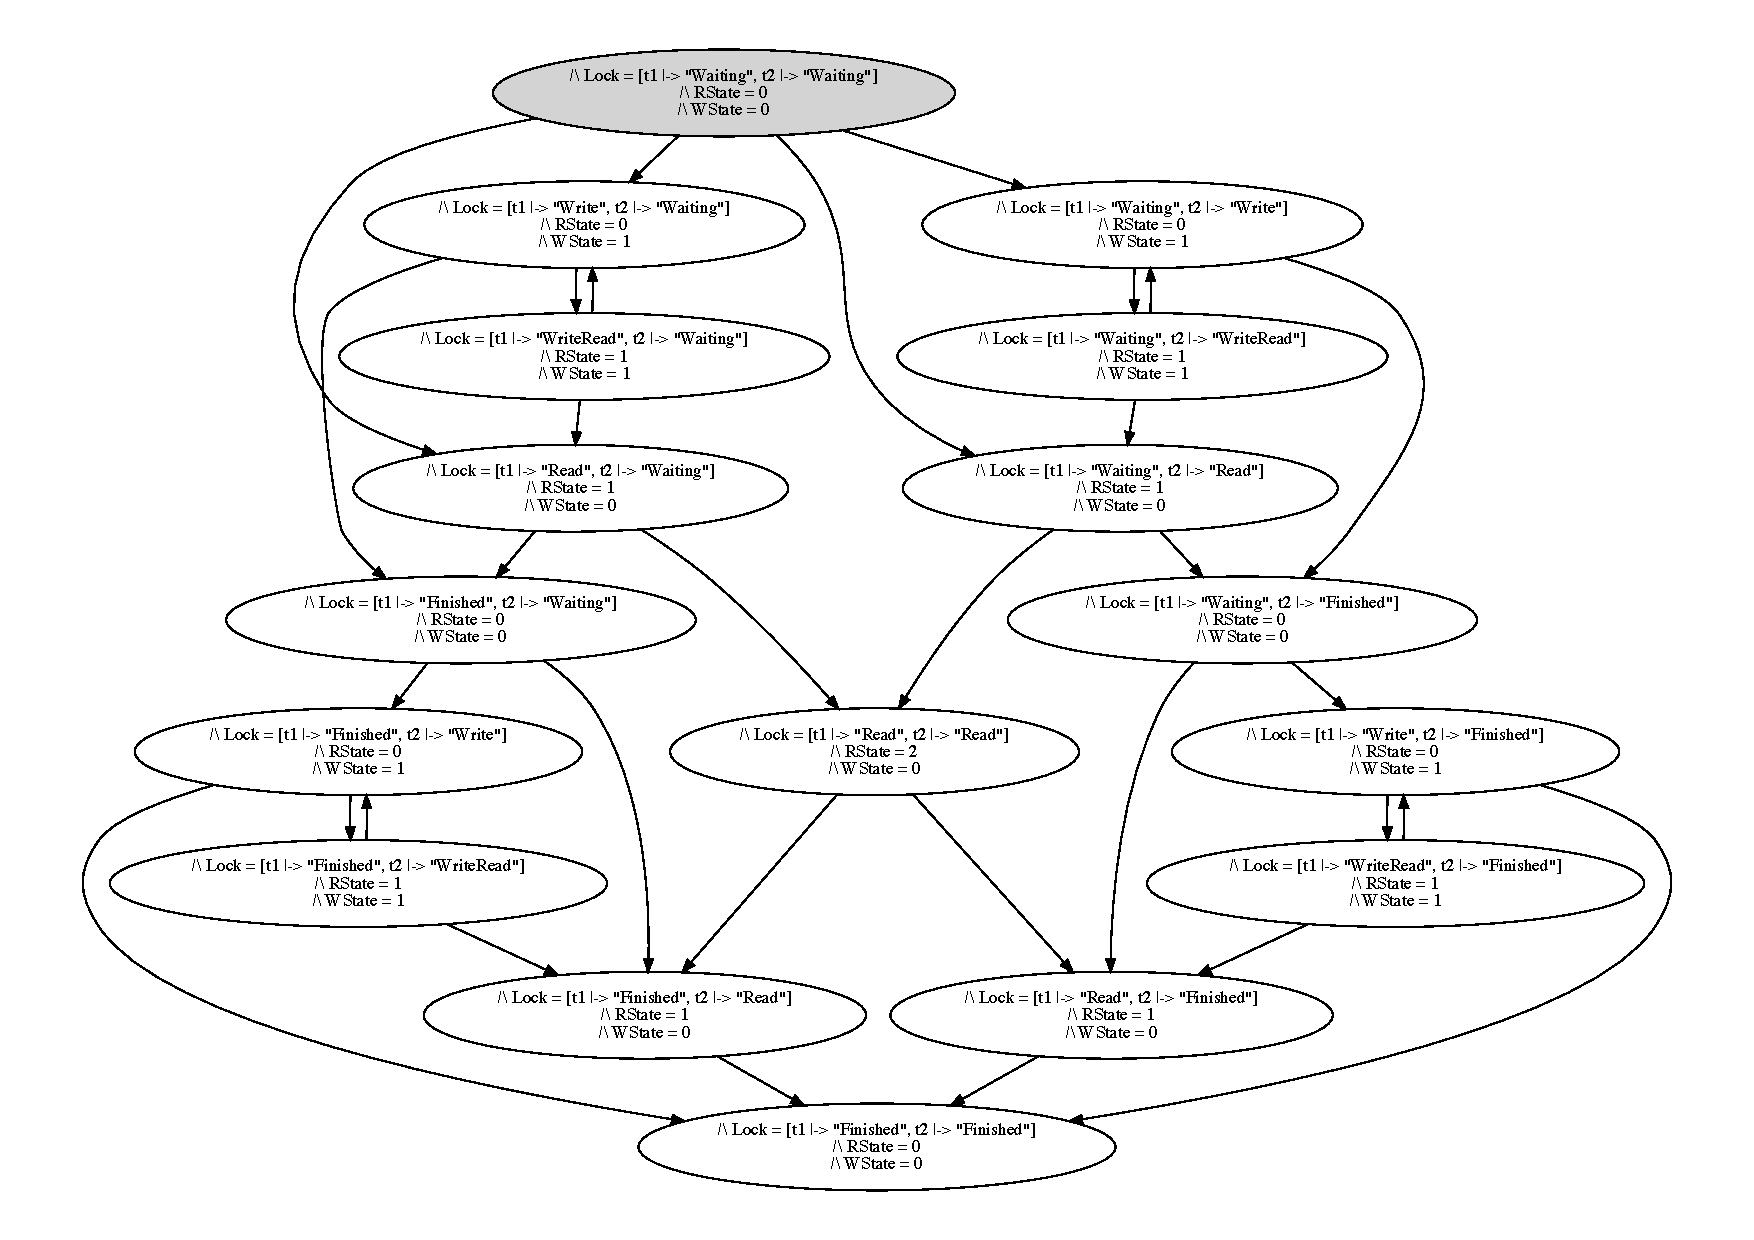
\includegraphics[scale=0.35,angle=90]{figures/aiorwlock_model}
      \end{center}
  \end{frame}
% --------------------------------------------------------------------------- %
  \begin{frame}{aiorwlock spec results}
    \begin{itemize}
      \item In fact bug reveled itself on specification phase, before
          running any models.
      \item Only three steps required to reproduce issue.
      \item First aio-libs project with formal verification!
    \end{itemize}
  \end{frame}
% --------------------------------------------------------------------------- %
  \section{Conclusions}
% --------------------------------------------------------------------------- %
  \begin{frame}{Limitations of Model-Checking}
    \begin{itemize}
      \item State space explosion number of states reachable by a system
          can quickly become huge, or even infinite
      \item Used as an adjunct to, not a replacement for, standard quality
          assurance methods
      \item Formal methods are not a panacea, but can increase confidence in
          a product’s reliability if applied with care and skill
    \end{itemize}
  \end{frame}
% --------------------------------------------------------------------------- %
\begin{frame}
    \vspace{1cm}
    \begin{center}{\Huge Questions?} \end{center}
    \begin{center} 
\includegraphics[scale=0.4]{figures/qrcode.png}\end{center}
    \begin{center}
        \href{http://github.com/jettify}{http://github.com/jettify}
    \end{center}
\end{frame}
% --------------------------------------------------------------------------- %
\appendix
\begin{frame}[allowframebreaks]{References}
    \bibliography{references}
    \bibliographystyle{abbrv}
\end{frame}
% --------------------------------------------------------------------------- %
\end{document}
% =========================================================================== %
